\documentclass{standalone}
\usepackage{tikz}
\usetikzlibrary{patterns, positioning}

\begin{document}
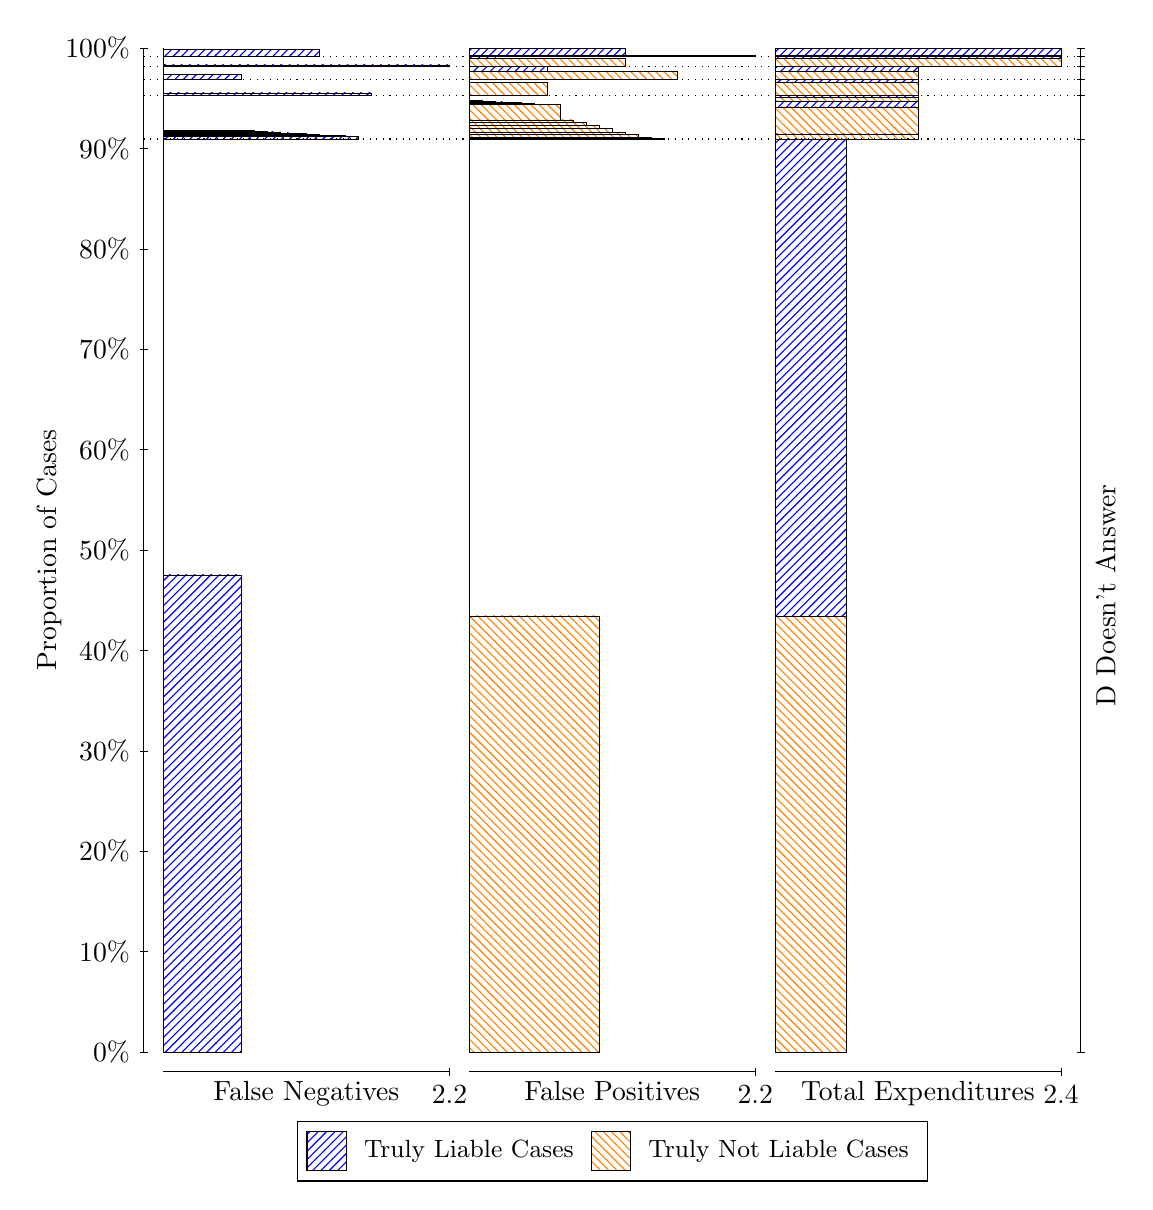
\begin{tikzpicture}
\draw[black, very thin] (1.5,1.75) -- (1.5,14.5);
\node[rotate=90, anchor=center] at (0.3, 8.125) {Proportion of Cases};
\draw[black, very thin] (1.45,1.75) -- (1.55,1.75);
\node[anchor=east] at (1.45, 1.75) {0\%};
\draw[black, very thin] (1.45,3.025) -- (1.55,3.025);
\node[anchor=east] at (1.45, 3.025) {10\%};
\draw[black, very thin] (1.45,4.3) -- (1.55,4.3);
\node[anchor=east] at (1.45, 4.3) {20\%};
\draw[black, very thin] (1.45,5.575) -- (1.55,5.575);
\node[anchor=east] at (1.45, 5.575) {30\%};
\draw[black, very thin] (1.45,6.85) -- (1.55,6.85);
\node[anchor=east] at (1.45, 6.85) {40\%};
\draw[black, very thin] (1.45,8.125) -- (1.55,8.125);
\node[anchor=east] at (1.45, 8.125) {50\%};
\draw[black, very thin] (1.45,9.4) -- (1.55,9.4);
\node[anchor=east] at (1.45, 9.4) {60\%};
\draw[black, very thin] (1.45,10.675) -- (1.55,10.675);
\node[anchor=east] at (1.45, 10.675) {70\%};
\draw[black, very thin] (1.45,11.95) -- (1.55,11.95);
\node[anchor=east] at (1.45, 11.95) {80\%};
\draw[black, very thin] (1.45,13.225) -- (1.55,13.225);
\node[anchor=east] at (1.45, 13.225) {90\%};
\draw[black, very thin] (1.45,14.5) -- (1.55,14.5);
\node[anchor=east] at (1.45, 14.5) {100\%};

\draw[black, very thin] (13.4,1.75) -- (13.4,14.5);
\draw[black, very thin] (13.35,1.75) -- (13.45,1.75);
\node[anchor=west] at (13.35, 1.75) {};
\draw[black, very thin] (13.35,13.345) -- (13.45,13.345);
\node[anchor=west] at (13.35, 13.345) {};
\draw[black, very thin] (13.35,13.894) -- (13.45,13.894);
\node[anchor=west] at (13.35, 13.894) {};
\draw[black, very thin] (13.35,14.1) -- (13.45,14.1);
\node[anchor=west] at (13.35, 14.1) {};
\draw[black, very thin] (13.35,14.267) -- (13.45,14.267);
\node[anchor=west] at (13.35, 14.267) {};
\draw[black, very thin] (13.35,14.39) -- (13.45,14.39);
\node[anchor=west] at (13.35, 14.39) {};
\draw[black, very thin] (13.35,14.5) -- (13.45,14.5);
\node[anchor=west] at (13.35, 14.5) {};

\draw[black, very thin, pattern color=blue, pattern=north east lines] (1.75,1.75) rectangle (2.7409,7.8081);
\draw[black, very thin, pattern color=orange, pattern=north west lines] (1.75,7.8081) rectangle (1.75,13.345);
\draw[black, very thin, pattern color=blue, pattern=north east lines] (1.75,13.345) rectangle (4.2273,13.381);
\draw[black, very thin, pattern color=blue, pattern=north east lines] (1.75,13.381) rectangle (4.0621,13.386);
\draw[black, very thin, pattern color=blue, pattern=north east lines] (1.75,13.386) rectangle (3.897,13.395);
\draw[black, very thin, pattern color=blue, pattern=north east lines] (1.75,13.395) rectangle (3.7318,13.403);
\draw[black, very thin, pattern color=blue, pattern=north east lines] (1.75,13.403) rectangle (3.5667,13.415);
\draw[black, very thin, pattern color=blue, pattern=north east lines] (1.75,13.415) rectangle (3.4015,13.422);
\draw[black, very thin, pattern color=blue, pattern=north east lines] (1.75,13.422) rectangle (3.2364,13.435);
\draw[black, very thin, pattern color=blue, pattern=north east lines] (1.75,13.435) rectangle (3.0712,13.442);
\draw[black, very thin, pattern color=blue, pattern=north east lines] (1.75,13.442) rectangle (2.9061,13.451);
\draw[black, very thin, pattern color=orange, pattern=north west lines] (1.75,13.451) rectangle (1.75,13.894);
\draw[black, very thin, pattern color=blue, pattern=north east lines] (1.75,13.894) rectangle (4.3924,13.93);
\draw[black, very thin, pattern color=orange, pattern=north west lines] (1.75,13.93) rectangle (1.75,14.1);
\draw[black, very thin, pattern color=blue, pattern=north east lines] (1.75,14.1) rectangle (2.7409,14.165);
\draw[black, very thin, pattern color=orange, pattern=north west lines] (1.75,14.165) rectangle (1.75,14.267);
\draw[black, very thin, pattern color=blue, pattern=north east lines] (1.75,14.267) rectangle (5.3833,14.287);
\draw[black, very thin, pattern color=orange, pattern=north west lines] (1.75,14.287) rectangle (1.75,14.39);
\draw[black, very thin, pattern color=blue, pattern=north east lines] (1.75,14.39) rectangle (3.7318,14.479);
\draw[black, very thin, pattern color=orange, pattern=north west lines] (1.75,14.479) rectangle (1.75,14.5);
\draw[black, very thin, pattern color=orange, pattern=north west lines] (5.6333,1.75) rectangle (7.2848,7.2871);
\draw[black, very thin, pattern color=blue, pattern=north east lines] (5.6333,7.2871) rectangle (5.6333,13.345);
\draw[black, very thin, pattern color=orange, pattern=north west lines] (5.6333,13.345) rectangle (8.1106,13.354);
\draw[black, very thin, pattern color=orange, pattern=north west lines] (5.6333,13.354) rectangle (7.9455,13.369);
\draw[black, very thin, pattern color=orange, pattern=north west lines] (5.6333,13.369) rectangle (7.7803,13.401);
\draw[black, very thin, pattern color=orange, pattern=north west lines] (5.6333,13.401) rectangle (7.6152,13.424);
\draw[black, very thin, pattern color=orange, pattern=north west lines] (5.6333,13.424) rectangle (7.45,13.478);
\draw[black, very thin, pattern color=orange, pattern=north west lines] (5.6333,13.478) rectangle (7.2848,13.516);
\draw[black, very thin, pattern color=orange, pattern=north west lines] (5.6333,13.516) rectangle (7.1197,13.555);
\draw[black, very thin, pattern color=orange, pattern=north west lines] (5.6333,13.555) rectangle (6.9545,13.586);
\draw[black, very thin, pattern color=orange, pattern=north west lines] (5.6333,13.586) rectangle (6.7894,13.788);
\draw[black, very thin, pattern color=blue, pattern=north east lines] (5.6333,13.788) rectangle (6.4591,13.797);
\draw[black, very thin, pattern color=blue, pattern=north east lines] (5.6333,13.797) rectangle (6.2939,13.805);
\draw[black, very thin, pattern color=blue, pattern=north east lines] (5.6333,13.805) rectangle (6.1288,13.817);
\draw[black, very thin, pattern color=blue, pattern=north east lines] (5.6333,13.817) rectangle (5.9636,13.824);
\draw[black, very thin, pattern color=blue, pattern=north east lines] (5.6333,13.824) rectangle (5.7985,13.836);
\draw[black, very thin, pattern color=blue, pattern=north east lines] (5.6333,13.836) rectangle (5.6333,13.894);
\draw[black, very thin, pattern color=orange, pattern=north west lines] (5.6333,13.894) rectangle (6.6242,14.064);
\draw[black, very thin, pattern color=blue, pattern=north east lines] (5.6333,14.064) rectangle (5.6333,14.1);
\draw[black, very thin, pattern color=orange, pattern=north west lines] (5.6333,14.1) rectangle (8.2758,14.201);
\draw[black, very thin, pattern color=blue, pattern=north east lines] (5.6333,14.201) rectangle (6.6242,14.267);
\draw[black, very thin, pattern color=orange, pattern=north west lines] (5.6333,14.267) rectangle (7.6152,14.37);
\draw[black, very thin, pattern color=blue, pattern=north east lines] (5.6333,14.37) rectangle (5.9636,14.39);
\draw[black, very thin, pattern color=orange, pattern=north west lines] (5.6333,14.39) rectangle (9.2667,14.411);
\draw[black, very thin, pattern color=blue, pattern=north east lines] (5.6333,14.411) rectangle (7.6152,14.5);
\draw[black, very thin, pattern color=orange, pattern=north west lines] (9.5167,1.75) rectangle (10.425,7.2871);
\draw[black, very thin, pattern color=blue, pattern=north east lines] (9.5167,7.2871) rectangle (10.425,13.345);
\draw[black, very thin, pattern color=orange, pattern=north west lines] (9.5167,13.345) rectangle (11.333,13.399);
\draw[black, very thin, pattern color=blue, pattern=north east lines] (9.5167,13.399) rectangle (11.333,13.411);
\draw[black, very thin, pattern color=orange, pattern=north west lines] (9.5167,13.411) rectangle (11.333,13.753);
\draw[black, very thin, pattern color=blue, pattern=north east lines] (9.5167,13.753) rectangle (11.333,13.827);
\draw[black, very thin, pattern color=orange, pattern=north west lines] (9.5167,13.827) rectangle (11.333,13.874);
\draw[black, very thin, pattern color=blue, pattern=north east lines] (9.5167,13.874) rectangle (11.333,13.894);
\draw[black, very thin, pattern color=orange, pattern=north west lines] (9.5167,13.894) rectangle (11.333,14.064);
\draw[black, very thin, pattern color=blue, pattern=north east lines] (9.5167,14.064) rectangle (11.333,14.1);
\draw[black, very thin, pattern color=orange, pattern=north west lines] (9.5167,14.1) rectangle (11.333,14.201);
\draw[black, very thin, pattern color=blue, pattern=north east lines] (9.5167,14.201) rectangle (11.333,14.267);
\draw[black, very thin, pattern color=orange, pattern=north west lines] (9.5167,14.267) rectangle (13.15,14.37);
\draw[black, very thin, pattern color=blue, pattern=north east lines] (9.5167,14.37) rectangle (13.15,14.39);
\draw[black, very thin, pattern color=orange, pattern=north west lines] (9.5167,14.39) rectangle (13.15,14.411);
\draw[black, very thin, pattern color=blue, pattern=north east lines] (9.5167,14.411) rectangle (13.15,14.5);
\draw[black, dotted] (1.5,13.345) -- (13.4,13.345);
\draw[black, dotted] (1.5,13.894) -- (13.4,13.894);
\draw[black, dotted] (1.5,14.1) -- (13.4,14.1);
\draw[black, dotted] (1.5,14.267) -- (13.4,14.267);
\draw[black, dotted] (1.5,14.39) -- (13.4,14.39);
\draw[black, very thin] (1.75,1.5) -- (5.3833,1.5);
\node[anchor=north] at (3.5667, 1.5) {False Negatives};
\draw[black, very thin] (5.3833,1.45) -- (5.3833,1.55);
\node[anchor=north] at (5.3833, 1.45) {2.2};

\draw[black, very thin] (5.6333,1.5) -- (9.2667,1.5);
\node[anchor=north] at (7.45, 1.5) {False Positives};
\draw[black, very thin] (9.2667,1.45) -- (9.2667,1.55);
\node[anchor=north] at (9.2667, 1.45) {2.2};

\draw[black, very thin] (9.5167,1.5) -- (13.15,1.5);
\node[anchor=north] at (11.333, 1.5) {Total Expenditures};
\draw[black, very thin] (13.15,1.45) -- (13.15,1.55);
\node[anchor=north] at (13.15, 1.45) {2.4};

\node[black, centered, rotate=90] at (13.72, 7.5476) {D Doesn't Answer};






\draw (7.449999999999999,1.5) node[draw=none] (baseCoordinate) {};
\begin{scope}[align=center]
        \matrix[scale=0.5, draw=black, below=0.5cm of baseCoordinate, nodes={draw}, column sep=0.1cm]{
            \node[rectangle, draw, minimum width=0.5cm, minimum height=0.5cm, pattern=north east lines, pattern color=blue] {}; &
            \node[draw=none, font=\small] (B) {Truly Liable Cases}; &
            \node[rectangle, draw, minimum width=0.5cm, minimum height=0.5cm, pattern=north west lines, pattern color=orange] {}; &
            \node[draw=none, font=\small] (B) {Truly Not Liable Cases}; \\
            };
\end{scope}

\end{tikzpicture}
\end{document}